\documentclass[a4paper,twoside,11pt]{memoir}

% This preamble is written by Amalie Stokholm with the help and inspiration from Steffen Videbæk, Mathias Rav, Rasmus Villemoes and Lars 'daleif' Madsen. 

% Check input
\usepackage[utf8]{inputenc}
\usepackage[T1]{fontenc}

% Fonts and microtype
\usepackage[danish,english]{babel}
\usepackage{csquotes}  % recommended when using babel
\usepackage{lmodern}
\usepackage[final]{microtype}

\usepackage{url}
\usepackage{xspace}

% Graphics
\usepackage{graphicx}

% Mathematics
\usepackage{amsmath}

% SI-units
\usepackage[detect-all]{siunitx}
	\sisetup{separate-uncertainty=true, % uses \pm instead of parenthesis
			per-mode=symbol}
% https://github.com/EdwinChan/latex-hacks/blob/master/astro.sty
\DeclareSIUnit\solarradius{\ensuremath{\mathit{R}_\odot}}
\DeclareSIUnit\solarmass{\ensuremath{\mathit{M}_\odot}}

% References
\usepackage{varioref}
\usepackage[colorlinks=true,
			allcolors=black
			]{hyperref}
\usepackage{cleveref}

% BibLaTeX, needs installation of Biber
\usepackage[style=authoryear-comp,
			backend=biber,
			hyperref=true,
			natbib=true,
            url=false,
            doi=false,
            isbn=false,
            uniquelist=false,
            uniquename=false,
            maxcitenames=2,mincitenames=1,
            ]{biblatex}
\bibliography{bachelor}

% Space in bibliography
\setlength\bibitemsep{1.5\itemsep}

% Replaces 'and' with ' &' http://tex.stackexchange.com/questions/68053/use-ampersand-in-citations-and-bibliography-in-biblatex
\renewcommand*{\finalnamedelim}{%
  \ifnumgreater{\value{liststop}}{2}{}{}%
  \addspace\&\space}

% Syntaxmarking: python
% Defining colors
\usepackage{color}
	\definecolor{deepblue}{rgb}{0,0,0.5}
	\definecolor{deepred}{rgb}{0.6,0,0}
	\definecolor{deepgreen}{rgb}{0,0.5,0}
\usepackage{listings}
% PDF accessibility support for literate listings
\usepackage{accsupp}
	\lstset{
			language=Python,
			basicstyle=\small\sffamily,
			keywordstyle=\color{deepblue},  
			emphstyle=\color{deepred},    
			stringstyle=\color{deepgreen},
			commentstyle=\color{red},        
			showstringspaces=false,
			columns=fullflexible,
			keepspaces=true,
			numbers=left,
			numbersep=20pt,
			numberstyle=\tiny,
			% escapeinside={$}{$},
			% mathescape=true,
			literate=
			{_}{%
			  \makebox[0pt][l]{%
			    \makebox[4pt][c]{%
			      \textcolor{white}{\_}}}%
			  \rule[-0.4pt]{4pt}{0.4pt}%
			}1
			{-}{%
			  % http://tex.stackexchange.com/a/18509/76220
			  % Use accessibility support to change what text
			  % is copied out of the PDF: ASCII hyphen
			  % instead of Unicode minus
			  \BeginAccSupp{
			    method=escape,
			    ActualText={-}
			  }%
			  $-$%
			  \EndAccSupp{}%
			}1
			{*}{%
			  % http://tex.stackexchange.com/a/18509/76220
			  % Use accessibility support to change what text
			  % is copied out of the PDF: ASCII hyphen
			  % instead of Unicode minus
			  \BeginAccSupp{
			    method=escape,
			    ActualText={*}
			  }%
			  $*$%
			  \EndAccSupp{}%
			}1
			{µ}{$\mu$}1
			{É}{{\'E}}1,
}
% The option to attach files (code)
\usepackage{attachfile}

% Filler text
\usepackage{lipsum}

% Fix-me
\usepackage[final]{fixme}
	\fxsetup{layout=footnote}

% Appendix i ToC
\renewcommand\cftappendixname{\appendixname~}

% Margins (with help from Steffen Videbæk)
\setlxvchars
\settypeblocksize{*}{1.03\lxvchars}{1.6181}
\setulmargins{*}{*}{1.6181}
\setlrmargins{*}{*}{1.6181}
\checkandfixthelayout[nearest] % needed in order for memoir to compile these settings correctly.

% TÅGEKAMMERET package allowing the right naming of tk
\pagestyle{headings}

% For default values, search for \makechapterstyle{default} in memoir.cls.
% Find memoir.cls with kpsewhich memoir.cls
\makechapterstyle{hangnumtight}{%
  \chapterstyle{hangnum}
  % hangnum by default has \beforechapskip=50pt 
  \setlength{\beforechapskip}{-20pt}
  % hangnum by default has \afterchapskip=40pt
  \setlength{\afterchapskip}{20pt}
}
\chapterstyle{hangnumtight}

% Macros
\newcommand{\projecttitle}{Interferometric and Asteroseismic Analysis of the Subgiant \mystar}
\newcommand{\projecttitledanish}{Interferometrisk og Asteroseismisk Analyse af Subkæmpestjernen \mystar}
\author{Amalie Louise Stokholm}
\date{\today}
\newcommand{\hdformat}[1]{HD~\@{#1}\xspace}
\newcommand{\mystar}{\hdformat{181096}}
\newcommand{\figref}[1]{Fig.\@~\ref{#1}\xspace}
\newcommand{\secref}[1]{Sec.\@~\ref{#1}\xspace}
\newcommand{\chapref}[1]{Chap.\@~\ref{#1}\xspace}
\newcommand{\tabref}[1]{Table~\ref{#1}\xspace}
\renewcommand{\eqref}[1]{Eq.\@~\ref{#1}\xspace}
\newcommand{\atlas}{\textsc{Atlas}\xspace}
\newcommand{\phoe}{\textsc{Phoenix}\xspace}
\newcommand{\stagger}{\textsc{Stagger}\xspace}
\newcommand{\kepler}{\emph{Kepler}\xspace}
\newcommand{\hipparcos}{Hipparcos\xspace}
\newcommand{\gaia}{Gaia\xspace}
\newcommand{\loli}{\textsc{L0L1}\xspace}
\newcommand{\lilii}{\textsc{L1L2}\xspace}
\newcommand{\aap}{Astronomy \& Astrophysics\xspace}
\newcommand{\araa}{Annual Review of Astronomy and Astrophysics\xspace}
\newcommand{\apj}{The Astrophysical Journal\xspace}

% Mathematics macros
\newcommand{\dx}[1]{\,\text{d}#1}
\newcommand{\vecb}[1]{\boldsymbol{{#1}}}
\newcommand{\teff}{T_{\text{eff}}}
\newcommand{\logg}{\log\,g}
\newcommand{\feh}{[\text{Fe}/\text{H}]}
\newcommand{\angdia}{\theta_\text{LD}}
\newcommand{\dn}{\Delta \nu}
\newcommand{\nmax}{\nu_{\text{max}}}

\selectlanguage{danish} 
\hyphenation{skala-relationen}
\selectlanguage{english}

% Includeonly
%\includeonly{frontpage}

\begin{document}
\frontmatter
% Forside
\begin{titlingpage}
 \projecttitle
 \newpage



% Colophone
\clearpage
\newgeometry{left=5cm,right=2cm,bottom=2cm}
\thispagestyle{empty} % fjerne evt. sidehoved og -fod
\small
%resten af teksten indenfor dette env skal være \small
\strut\vfill % pres alt ned i bunden af siden
\begin{flushleft}
\projecttitle \par \projecttitledanish \par \vspace{11 pt}
Amalie Louise Stokholm, 2016 \par
Bachelor's project written under supervision of Victor~Silva~Aguirre and Timothy~White at Stellar~Astrophysics~Centre, Department~of~Physics~and~Astronomy, Aarhus~University \par\vspace{11 pt}
This document is typeset with \LaTeX\xspace using the \textsf{memoir} class. The text is set with \emph{Latin~Modern} in 11 point size. The choice of layout with the limit of 66 characters per line is quite deliberate since the author believes that the chosen layout improves readability, and with approximately 36 lines per page it adheres to the requirement that a page of text contains approximately 2400 characters. When the empty pages and extra white space are taken into account, the project is less than 30 pages. \par
\vspace{11 pt}
Printed at Aarhus~University \par\vspace{11 pt}
\emph{Cover page: The large upper figure shows an area of the sky in the constellation \emph{Cygnus}. The image is an infra-red picture constructed from three different bands, false coloured in three colours: J band (\SI{1.2}{\micro\meter}) coloured blue, H band (\SI{1.6}{\micro\meter}) coloured green, and K$_s$ band (\SI{2.2}{\micro\meter}) coloured red. This image is from the Two Micron All Sky Survey (2MASS) \citep{mass} found using the Aladin Sky Atlas \citep{aladin}. \\ The magnified part shows the star \mystar, which is the object of interest in this study.} 
\end{flushleft}
\end{titlingpage}
\restoregeometry % Front page & colophone
\pagenumbering{roman}
\subsection*{Abstract}
{\small In this bachelor's project, an interferometric and asteroseismic analysis of the subgiant star \mystar is presented. The aim of the project is to calculate the radius of this star using interferometry and then compare the result with a radius determined from asteroseismology. 

The interferometric analysis uses measurements from the CHARA array. A calibration procedure is performed and the limb-darkening coefficient is estimated using tables from stellar model atmospheres. The interferometric angular diameter is calculated from the fit to the measurements, and combined with the \hipparcos parallax, the linear radius of the star is found to be $R = \SI{2.07 \pm 0.04}{\solarradius}$. Using the interferometric angular diameter, the effective temperature of \mystar is determined to be $\teff = \SI{6211 \pm 91}{\kelvin}$.

The asteroseismic analysis uses short-cadence data from the \kepler mission. The determined asteroseismic parameters are used in one of the asteroseismic scaling relations to find the radius. The radius of \mystar is computed to be 
$R = \SI{2.20 \pm 0.05}{\solarradius}$.

The difference between the two radii is $\SI{2.03}{\sigma}$, which is significant.
It could be due to an assumption about the shape of the oscillation profile used in the asteroseismic analysis being wrong,
or it could be a systematic deviation of the scaling relation for this type of star. \par
}
\subsection*{Resumé}
\selectlanguage{danish} 
{\small Dette bachelorprojekt gennemgår en interferometrisk og asteroseismisk analyse af subkæmpestjernen \mystar. Formålet med projektet er at beregne stjernens radius ved brug af interferometri og sammenligne resultatet med en radius fundet ved asteroseismologi. 

Den interferometriske analyse bruger målinger foretaget på det sammenkoblede interferometer CHARA. Et kalibreringsprogram anvendes, og ud fra modeller af stjerneatmosfærer bestemmes randformørkelseskoefficienten. Den interferometriske vinkeldiameter findes fra et fit til målingerne, og når den kombineres med parallaksen målt af Hipparcos, bestemmes den lineære radius af stjernen til $R = \SI{2.07 \pm 0.04}{\solarradius}$. Ved at bruge vinkeldiameteren estimeres den effektive temperatur til at være $\teff = \SI{6211 \pm 91}{\kelvin}$.

Den asteroseismiske analyse bruger kort-kadence data fra \kepler-missionen. De herfra fundne asteroseismiske parametre bliver brugt i en af de asteroseismiske skalarelationer til at finde radius. Radius af \mystar findes til at være $R = \SI{2.20 \pm 0.05}{\solarradius}$. 

De to radier afviger med $\SI{2.03}{\sigma}$, hvilket er en betydelig forskel. Det kan skyldes, at antagelsen om formen af oscillationsprofilen brugt i den asteroseismiske analyse kan være forkert, eller det kan udtrykke, at resultater fra de asteroseismiske skalarelationer afviger systematisk for denne type stjerne. \par
}
\clearpage
\selectlanguage{english} 
\section*{Acknowledgements}
\vspace{-5pt}
Numerous people have contributed and helped with this project in one way or another, and I would like to thank all of them. I would like to thank my supervisors Victor~Silva~Aguirre and Tim~White for guiding me through the entire process and for helping me sculpt the project. I would also like to thank them for allowing me to continue to work with this star for the upcoming months in order for me to learn new and exciting methods.

I would like to thank Mathias Rav sincerely for providing me with his unfailing support and love, but also for his  valuable help and comments on this thesis.

I would also like to thank Jakob Rørsted Mosumgaard and Kenneth Lund Kjærgaard
for participating in many rich discussions and for giving helpful suggestions during this project, but also for sharing their interest in and enthusiasm for astronomy in the time we have known each other.


\clearpage % Abstract (in english and danish), a preface and the acknowledgements
\tableofcontents*
\mainmatter
\chapter{Introduction}
Understanding the evolution and structure of stars is one of the main challenges in modern astrophysics. Fundamental properties of stars such as radius, mass and temperature need to be measured in order to compare them to predictions made using stellar models. 
Advances in understanding stars are driven by ever more precise measurements which can test the theories behind the models. Interferometry and asteroseismology are amongst the most powerful tools we have for this. Interferometry allows an almost-direct measurement of the physical size of star, although it can only be applied to the brightest stars. Asteroseismology enables us to infer stellar properties by measuring the variety of waves travelling through the stellar interior. 
Ideally both methods can be used in order to find the constraints needed for stellar modelling and thus to test -- and improve -- our current models of stellar structure and evolution.

The aim of this project is to determine the radius of a subgiant star from interferometry and then compare with a radius determined from asteroseismology. 
The subgiant star of interest is \mystar. This star has not been the subject of detailed studies before, but has mostly been used as a comparison star in spectroscopy and photometry \citep{schiller1988photometric,ferrero2004magnetic}.
The entire process from raw data to radius of the star using both asteroseismology and interferometry will be explained and discussed in this project.

In this chapter, the theoretical background for interferometry and asteroseismology is introduced. 
Sec.~\ref{sec:principleinterferometry} present the basics of interferometry.

\vspace{-5pt}
\section{The Principle of Interferometry}
\label{sec:principleinterferometry}
\vspace{-5pt}
Interferometry is an observational method in which the interference of electromagnetic waves is used to obtain the greatest possible angular resolution. 
%The underlying principle is the wave nature of light and the interference of these waves. 
A full and detailed review is given by  \citet{lawson2000principles} and \citet{monnier2003optical} upon which this section is based.
\plainbreak1
The fundamental principle of the interference of light can be nicely illustrated by Young's double slit experiment. In this experiment, monochromatic light from a distant point source illuminates a plate with two parallel, narrow slits separated by a distance~$B$.
The light travels through this double-slit assembly and towards the detection screen on the other side. According to Huygens's principle, every point of the wave front may be considered as a source of secondary spherical wavelets with a speed equal to the propagation speed of the wave. These wavelets interfere with one another, creating an interference pattern on the detection screen.
\begin{figure}
	\centering
	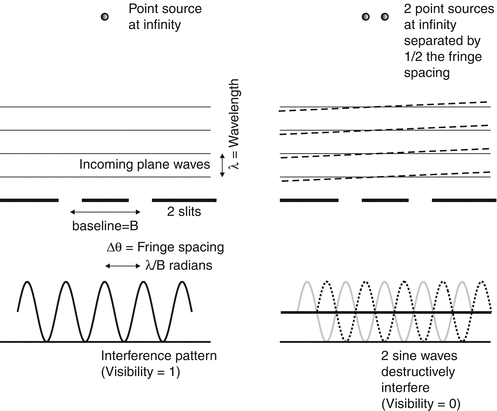
\includegraphics[width=1\linewidth]{./figures/fig72monnier2003-cropped}
	\caption{Two scenarios: the case of a single point-like light source, and the case of two point sources, separated by an angle of half the fringe spacing. The visibility is one and zero respectively due to interference. Figure from \citet{monnier2003optical}.}
	\label{fig:fig72monnier2003}
\end{figure}
Because the wavelets all have the same frequency, the resulting pattern is determined only by the phase difference between two waves. If the two waves are in phase (anti-phase) when they hit the detection screen, they will interfere constructively (destructively) and produce a bright (dark) patch. 
%If the two waves are in anti-phase, destructive interference will occur and appear as a dark patch. 
From the grating equation, the angular spacing between the bright and dark spots $\Delta \Theta$ can be approximated as
\begin{equation}
\label{eq:angularspacing}
\Delta \Theta \approx \frac{\lambda}{B},
\end{equation}
where $\lambda$ is the wavelength of the light and $B$, as mentioned earlier, denotes the distance between the slits. This distance is also called the baseline, hence the symbol $B$. 
%Imagine the scenario in which a second point-like light source of equal brightness as the first also illuminates the plate and this second light source is placed at exactly half a fringe spacing,  ${\Delta \Theta}/{2} = {\lambda}/{2 B}$, in angular distance from the first light source as seen from the plate as shown in \figref{fig:fig72monnier2003}. 
%In two-telescope interferometry, the two slits in Young's experiment are replaced by two telescopes, and we could imagine two point-like sources as two stars far away. 
In \figref{fig:fig72monnier2003}, a second point source of equal brightness as the first is placed at half a fringe spacing,  ${\Delta \Theta}/{2} = {\lambda}/{2 B}$, in angular distance from the first light source as seen from the plate. 
The combined light from these point sources will interfere destructively at all points  on the screen since the fringes are in exact anti-phase, and therefore, no contrast between bright and dark spots is visible.
%Therefore the combined light will show no contrast between bright and dark spots; the detection screen will just be evenly illuminated. 

This suggests that the contrast between the dark and bright patches in the interference pattern at a given wavelength and baseline is directly related to the structure of the observed object. 
The pattern is affected by the angular separation of two point sources or the angular extent of a single extended object. More precisely, the fringe contrast or the visibility $V$ can be defined as the ratio between the fringe amplitude (i.e.\@ half the difference between the maximum and minimum intensity $ (I_{\text{max}}-I_{\text{min}})/2$) and the average intensity:
\begin{equation}
V = \frac{I_{\text{max}}-I_{\text{min}}}{I_{\text{max}}+I_{\text{min}}} = \frac{\text{Amplitude}}{\text{Average intensity}}. 
\end{equation}
In the case of total constructive (destructive) interference, the visibility is one (zero).
%The Van Cittert-Zernike theorem relates more generally the complex fringe visibility $Q$ to a unique spatial Fourier transform of the intensity distribution of an object, see \citet{bradt2004astronomy}.
% $I(\vecb{\alpha})$:
%\begin{equation}
%Q(\vecb{\beta}) = \frac{\int I(\vecb{\alpha}) e^{-2\pi\vecb{\alpha}\vecb{\beta}}\dx{\vecb{\alpha}}}{\int I(\vecb{\alpha})\dx{\vecb{\alpha}}},
%\end{equation}
%where $\vecb{\alpha}$ is a given set of two-dimensional image coordinates and $\vecb{\beta}$ is the so-called spatial frequency, defined as the projected baseline vector $B$ (projection of the vector from telescope a to telescope b) scaled by the wavelength of the observation $\lambda$. A detailed review can be found in \citet{bradt2004astronomy}.
If the fringe visibility of an object is measured at different spatial frequencies, the spatial structure of the light source may be exposed \citep{van1934wahrscheinliche,zernike1938concept}. The spatial frequency $\beta$ is defined as the projected baseline $B$ in units of the wavelength $\lambda$
\begin{equation}
\label{eq:spatialfreq}
\beta = \frac{B}{\lambda}.
\end{equation} 
If the object in question is a star, measuring $V$ as a function of $\beta$ makes it possible to measure the angular diameter of the star. 

\printbibliography
\appendix
\include{appendix}
\end{document}